\documentclass[12pt]{article}
\usepackage[utf8]{inputenc}
\usepackage{graphicx}
\usepackage{multicol}
\usepackage{listings}
\usepackage{amsmath}
\graphicspath{ {./images/} }
\usepackage{amssymb}
\usepackage[htt]{hyphenat}

\usepackage{hyperref}
\hypersetup{
    colorlinks=true,
    linkcolor=blue,
    filecolor=magenta,      
    urlcolor=cyan,
}

\usepackage{xcolor}

\definecolor{codegreen}{rgb}{0,0.6,0}
\definecolor{codegray}{rgb}{0.5,0.5,0.5}
\definecolor{codepurple}{rgb}{0.58,0,0.82}
\definecolor{backcolour}{rgb}{0.95,0.95,0.92}
\definecolor{codeorange}{rgb}{1,0.64,0}

\lstdefinestyle{mystyle}{
    backgroundcolor=\color{backcolour},   
    commentstyle=\color{codegreen},
    keywordstyle=\color{magenta},
    numberstyle=\tiny\color{codeorange},
    stringstyle=\color{codepurple},
    basicstyle=\ttfamily\footnotesize,
    breakatwhitespace=false,         
    breaklines=true,                 
    captionpos=b,                    
    keepspaces=true,                 
    numbers=left,                    
    numbersep=5pt,                  
    showspaces=false,                
    showstringspaces=false,
    showtabs=false,                  
    tabsize=2
}

\lstset{style=mystyle, breaklines=true, postbreak=\mbox{\textcolor{red}{$\hookrightarrow$}\space}}

\title{\vspace{-1cm}Symbolic Computing using SymPy\\
\large Assignment 7\\
\large EE2703 - Applied Programming Lab}
\author{Abhigyan Chattopadhyay \\
EE19B146}
\date{20th April 2021}
\usepackage[margin=0.75in]{geometry}

\begin{document}
\maketitle
\tableofcontents
\pagebreak
\section{The Problem at Hand}
We will be using Symbolic computing to make it easier to calculate transfer functions of Active filters and work with them much more easily.

\section{Active Filters}
Active filters make use of Operational Amplifiers to improve the filtering quality and allow for controllable bandwidth.

\begin{center}
    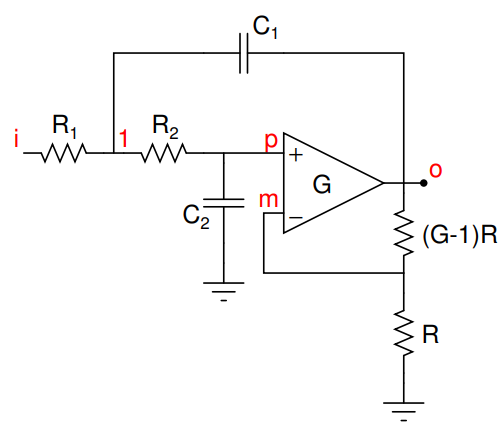
\includegraphics[scale=1]{images/ckt1.png}
\end{center}

The above circuit behaves as an active lowpass filter. We will now analyze the circuit in the Laplace domain manually first:
\begin{equation}
    V_m = \frac{V_o}{G}
\end{equation}
\begin{equation}
    V_1 \left(\frac{1}{R_1} + \frac{1}{R_2} + s C_1\right) - \frac{V_i}{R_1} - s C_1 V_o - \frac{V_p}{R_2} = 0
\end{equation}
\begin{equation}
    V_p = \frac{V_1}{1+s C_2 R_2}
\end{equation}
\begin{equation}
    V_o = G(V_p - V_m)
\end{equation}

We can convert these linear equations into a Matrix equation to simplify the calculation:
\begin{equation}
\begin{bmatrix}
    0 & 0 & 1 & -\frac{1}{G} \\
    -\frac{1}{1+s C_2 R_2} & 1 & 0 & 0 \\
    0 & -G & G & 1 \\
    \frac{1}{R_2}+\frac{1}{R_1}+sC_1 & -\frac{1}{R_2} & 0 & -s C_1
\end{bmatrix}
\begin{bmatrix}
    V_1 \\
    V_p \\
    V_m \\
    V_o
\end{bmatrix}
=
\begin{bmatrix}
    0 \\
    0 \\
    0 \\
    \frac{V_i}{R_1}
\end{bmatrix}
\end{equation}
Or: $Av = b$

Now, we can solve the matrix equation for any given input $V_i$ to obtain $v$.

Later on, we will be using a highpass filter which is essentially same as solving the lowpass filter, but we will have different equations for it.

\begin{center}
    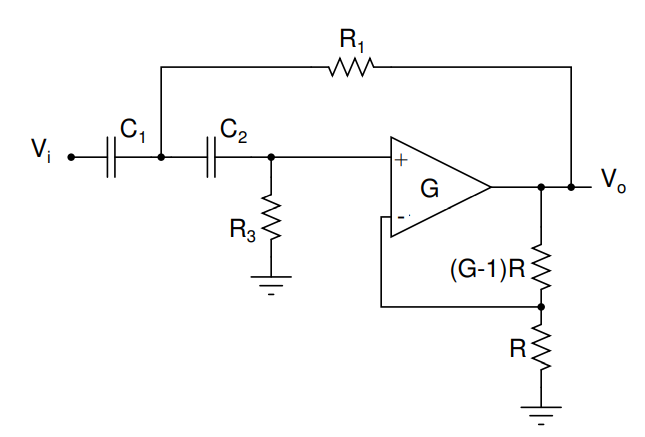
\includegraphics[scale=1]{images/ckt2.png}
\end{center}

Equations for the highpass filter are:

\begin{equation}
    V_m = \frac{V_o}{G}
\end{equation}
\begin{equation}
    V_1 \left(sC_2 + \frac{1}{R_1} +sC_1 \right) - s C_1 V_i - \frac{V_o}{R_1} - s C_2 V_p = 0
\end{equation}
\begin{equation}
    V_p = \frac{V_1}{1+\frac{1}{s C_2 R_3}}
\end{equation}
\begin{equation}
    V_o = G(V_p - V_m)
\end{equation}

\begin{equation}
\begin{bmatrix}
    0 & 0 & 1 & -\frac{1}{G} \\
    -\frac{1}{1+\frac{1}{s C_2 R_3}} & 1 & 0 & 0 \\
    0 & -G & G & 1 \\
    \frac{1}{R_1}+sC_1 + sC_2 & -s C_2 & 0 & -\frac{1}{R_1}
\end{bmatrix}
\begin{bmatrix}
    V_1 \\
    V_p \\
    V_m \\
    V_o
\end{bmatrix}
=
\begin{bmatrix}
    0 \\
    0 \\
    0 \\
    s C_1 V_i
\end{bmatrix}
\end{equation}
Again, this is also expressible in the form $Av=b$.

Now, we will set up these problems using SciPy and SymPy to work through them and get their responses to various inputs.
\pagebreak
\section{Solutions to the Given Problems}
\subsection{Pre-requisite functions}

We will create a function to convert from the SymPy format to the SciPy TransferFunctionContinuous class so that we can plot the values easily.

Code:
\begin{lstlisting}[language=Python]
def sympy_to_lti(symp, s=symbols('s')):
    """Convert Sympy transfer function polynomial to Scipy TransferFunctionContinuous"""
    n, d = fraction(symp)  # expressions of numerator and denominator
    p_num_den = poly(n, s), poly(d, s)
    num, den = p_num_den[0].all_coeffs(), p_num_den[1].all_coeffs()
    return sp.lti(np.array(num,dtype=float), np.array(den,dtype=float))
\end{lstlisting}

Next we will create the Low Pass Butterworth Filter and plot its frequency response using the lambdify command:

\begin{lstlisting}[language=Python]
# Setting up the Low Pass Butterworth Filter
s = symbols('s')
G = 1.586
R1 = R2 = 1e4
C1 = C2 = 1e-9
V1 = 1
A = Matrix([[0,0,1,-1/G],[-1/(1+s*R2*C2),1,0,0],[0,-G,G,1],[-1/R1 -1/R2 -s*C1, 1/R2, 0, s*C1]])
b = Matrix([0,0,0,-V1/R1])
V = A.inv()*b

# Plotting its Frequency Response
Vo = V[3]
H = sympy_to_lti(Vo)
omega = np.logspace(0,8,801)
ss = 1j*omega
hf = lambdify(s, Vo, 'numpy')
v = hf(ss)
plt.figure(0)
plt.loglog(omega,abs(v))
plt.xlabel(r"$\omega \rightarrow$")
plt.ylabel(r"$|H(j \omega)|\rightarrow$")
plt.grid(True)
plt.title("Magnitude Response of Butterworth Lowpass Filter")
plt.savefig("images/fig0",dpi=1000)
plt.show()
\end{lstlisting}
\pagebreak
Graph obtained:
\begin{center}
    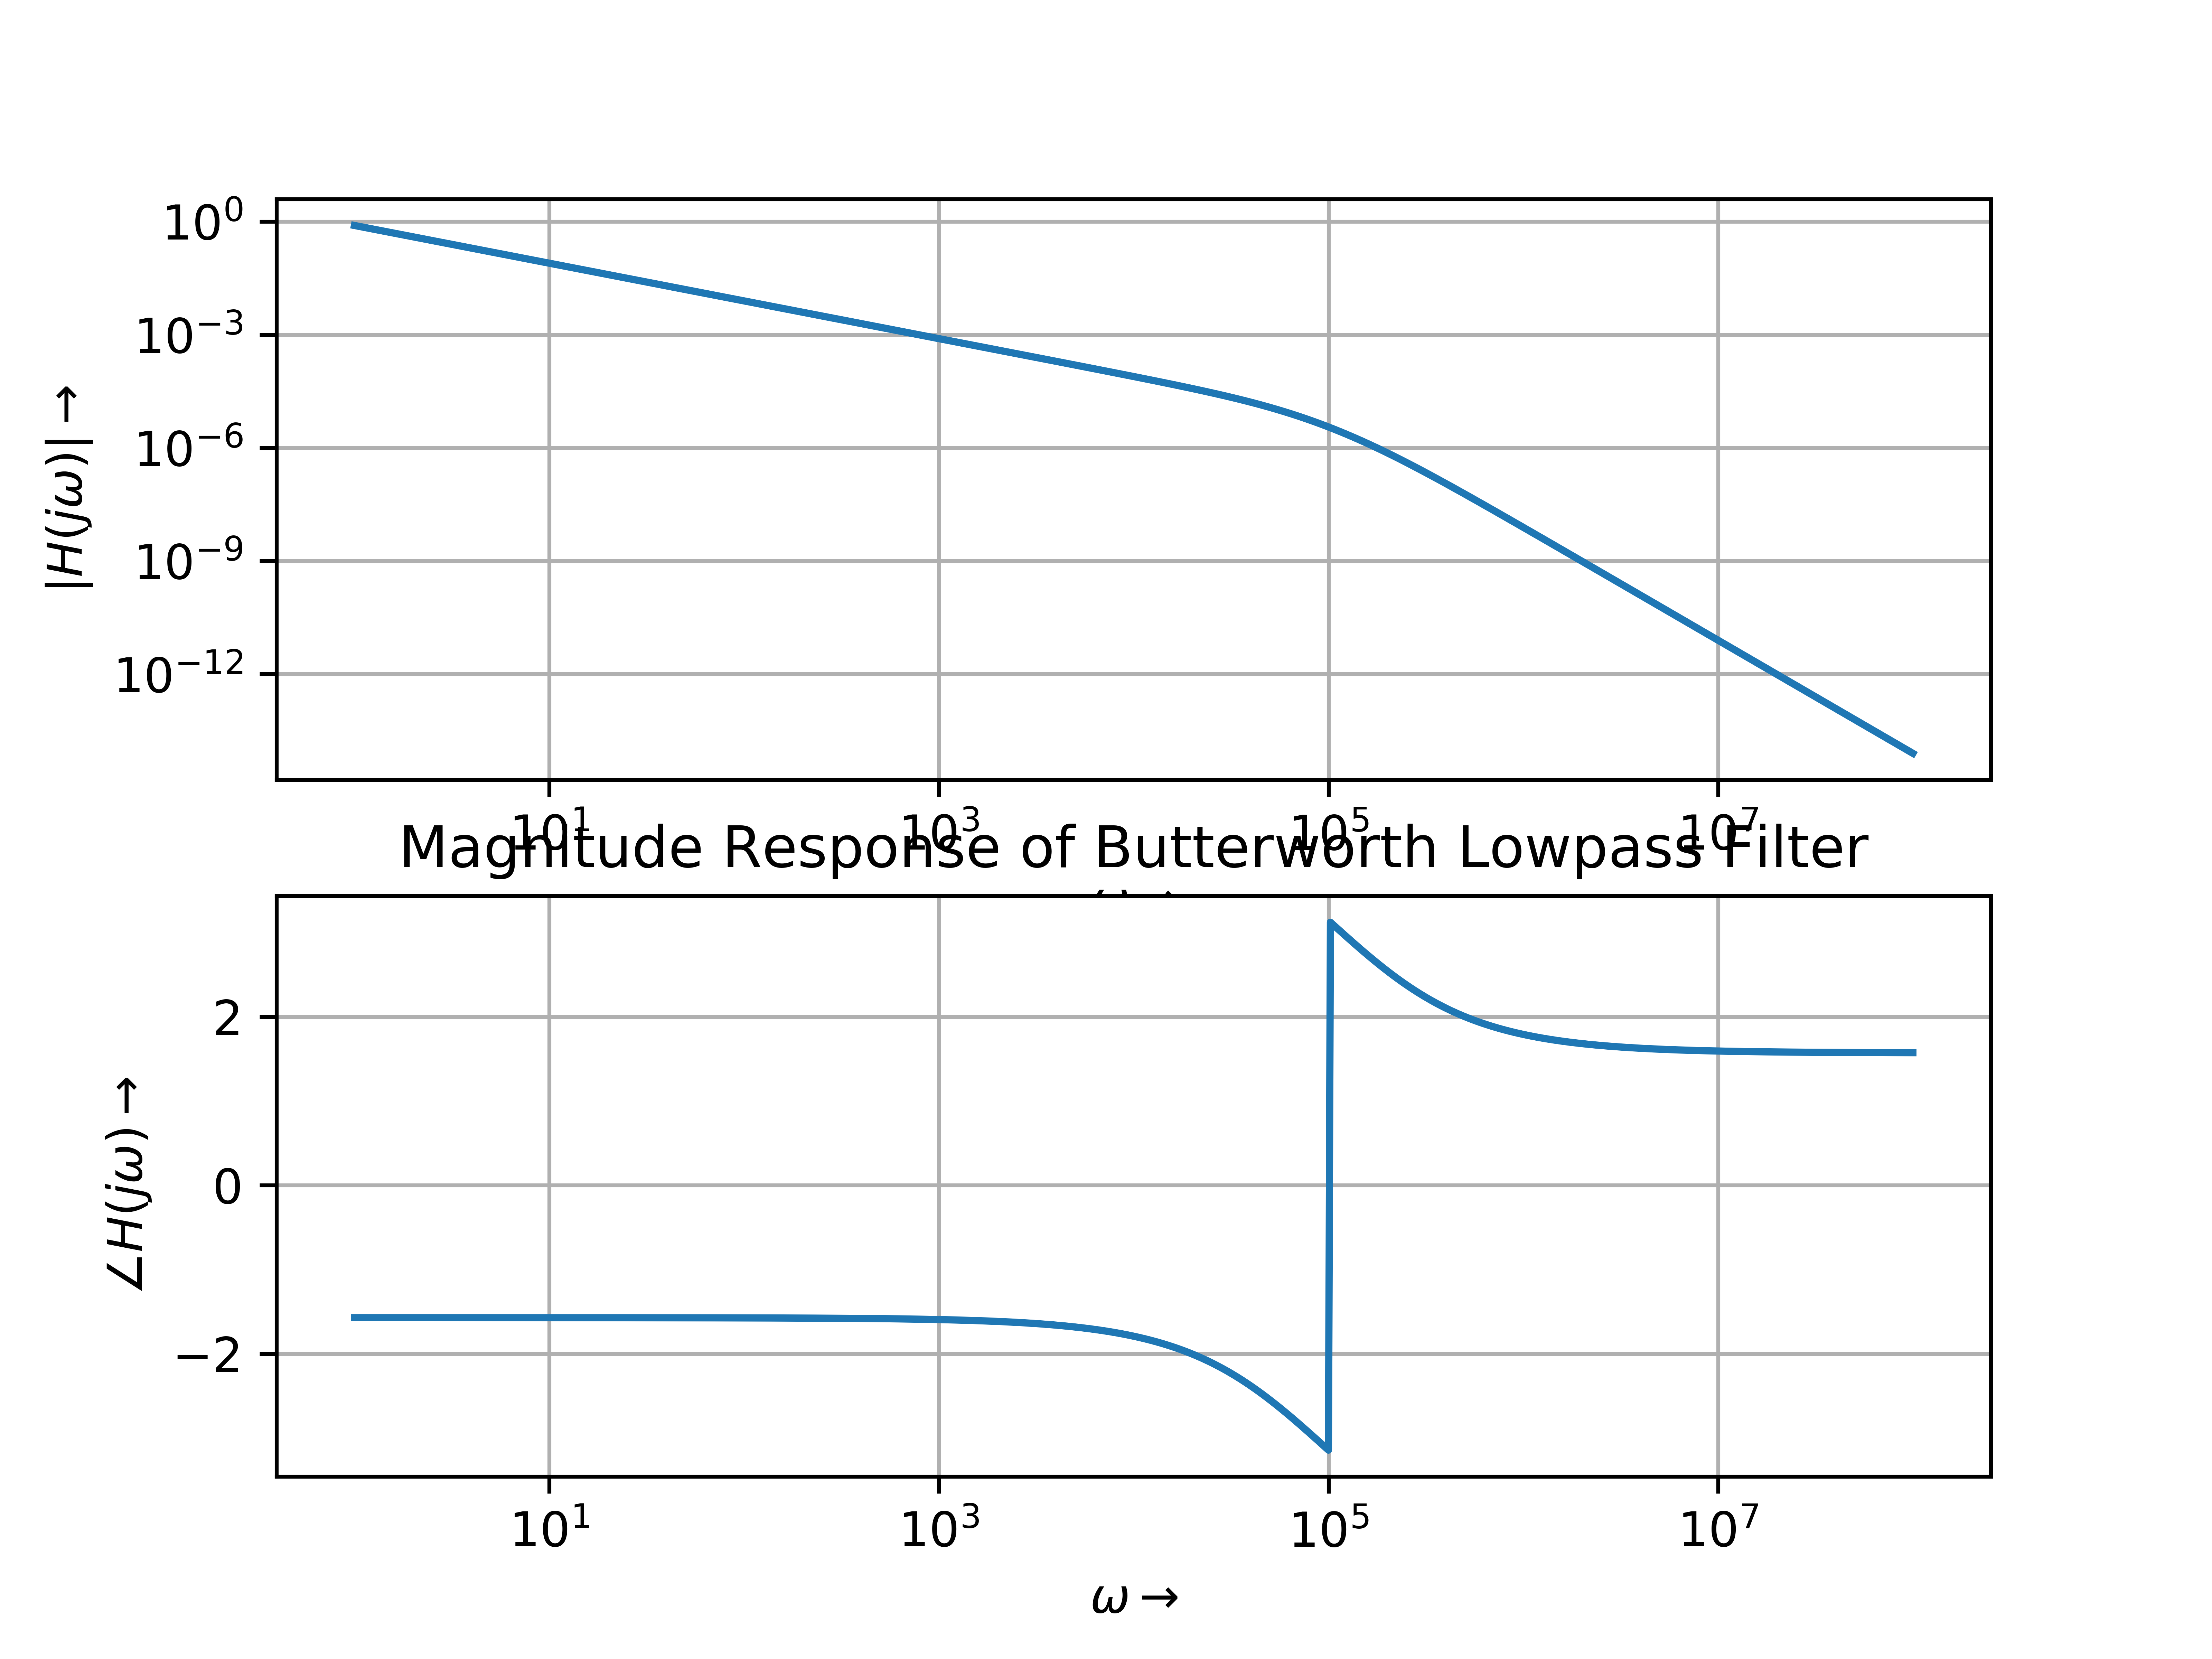
\includegraphics[scale=0.8]{images/fig0.png}
\end{center}

\pagebreak
\subsection{Question 1}
Code:
\begin{lstlisting}[language=Python]
t = np.linspace(0,0.001,1000)
t1,Vo1 = sp.step(H,T=t)

plt.figure(1)
plt.plot(t1,Vo1,"-",label=r"$V_0$")
plt.xlabel(r't$\rightarrow$')
plt.ylabel(r'$V_{o}\rightarrow$')
plt.title('Lowpass Butterworth Filter Step Response')
plt.legend(loc='upper right')
plt.grid(True)
plt.savefig("images/fig1",dpi=1000)
plt.show()
\end{lstlisting}
Graph obtained:
\begin{center}
    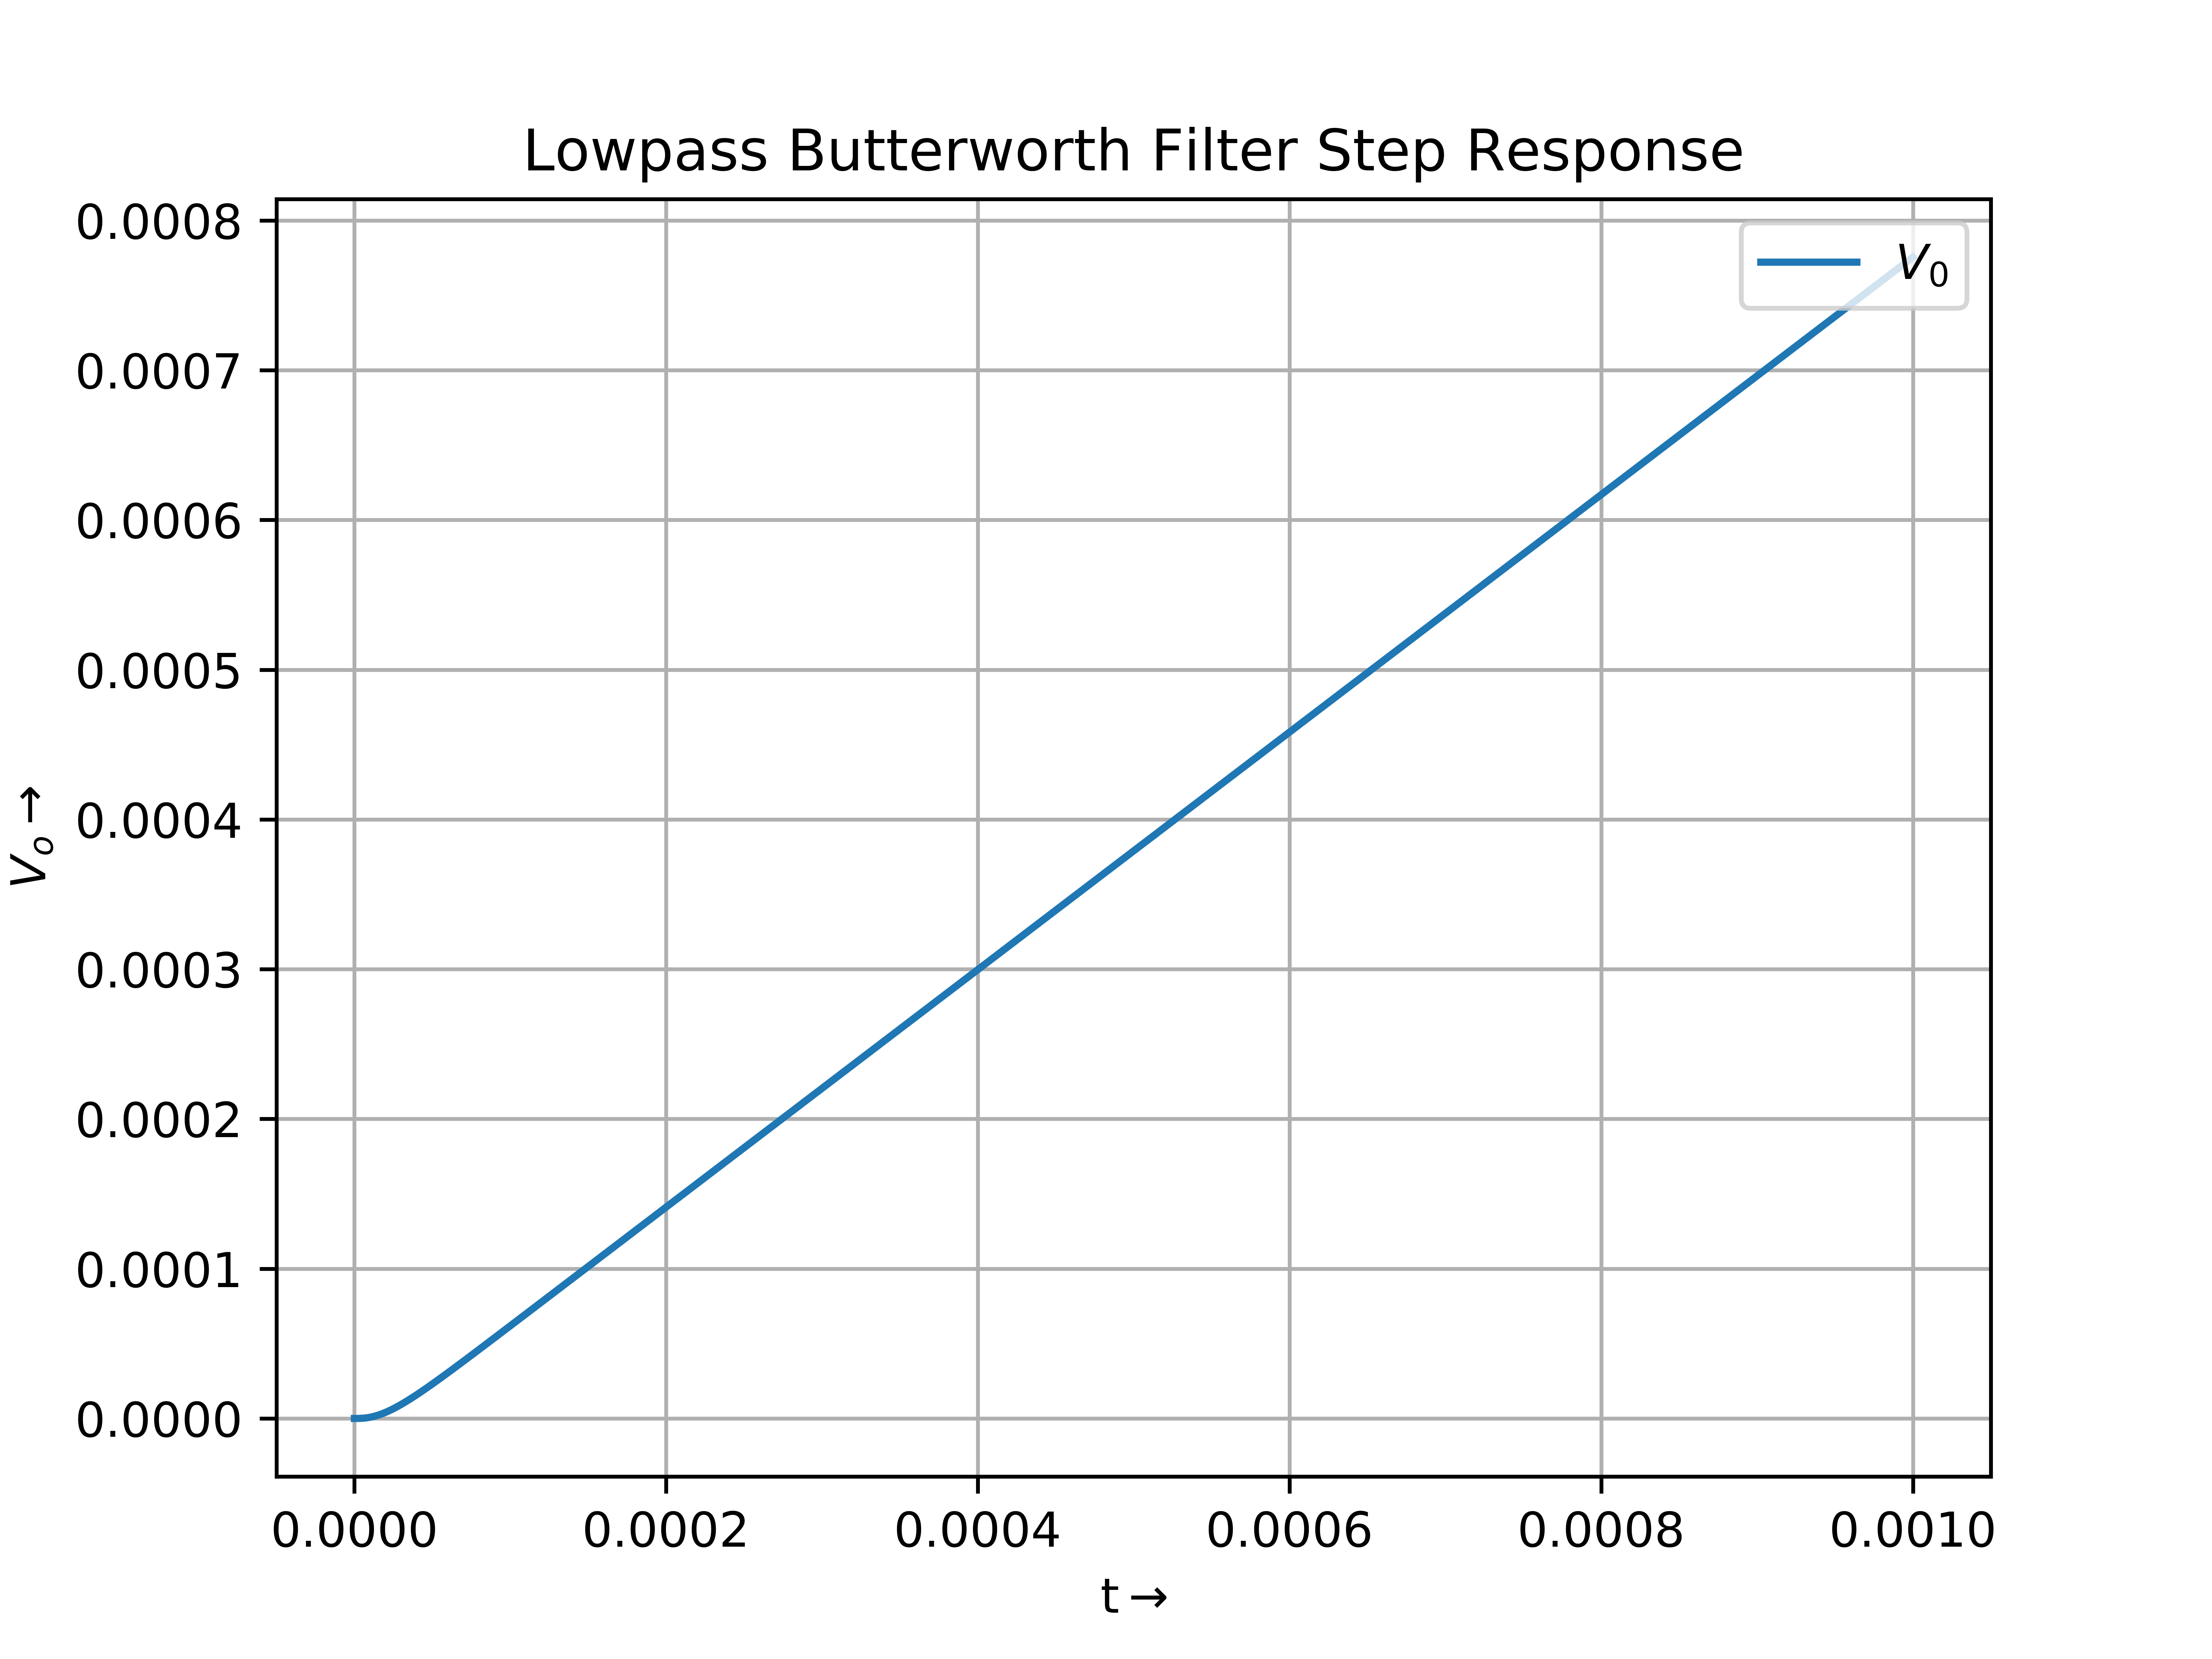
\includegraphics[scale=0.8]{images/fig1.png}
\end{center}
\pagebreak
\subsection{Question 2}

Now we will plot the response of Lowpass Butterworth filter to a mixed frequency sinusoid:

\begin{lstlisting}[language=Python]
t = np.linspace(0,0.01,100000)
Vi = np.multiply((np.sin(2000*np.pi*t)+np.cos(2000000*np.pi*t)),np.heaviside(t,0.5))
Vo = sp.lsim(H,Vi,T=t)
plt.figure(2)
plt.plot(Vo[0],Vi,label=r'$V_{in}$')
plt.plot(Vo[0],Vo[1],label=r'$V_{out}$')
plt.xlabel(r't$\rightarrow$')
plt.ylabel(r'V$\rightarrow$')
plt.title("Filter Response for Mixed Frequency Sinusoid")
plt.legend(loc="upper right")
plt.savefig("images/fig2", dpi=1000)
plt.show()
\end{lstlisting}
Graph obtained:
\begin{center}
    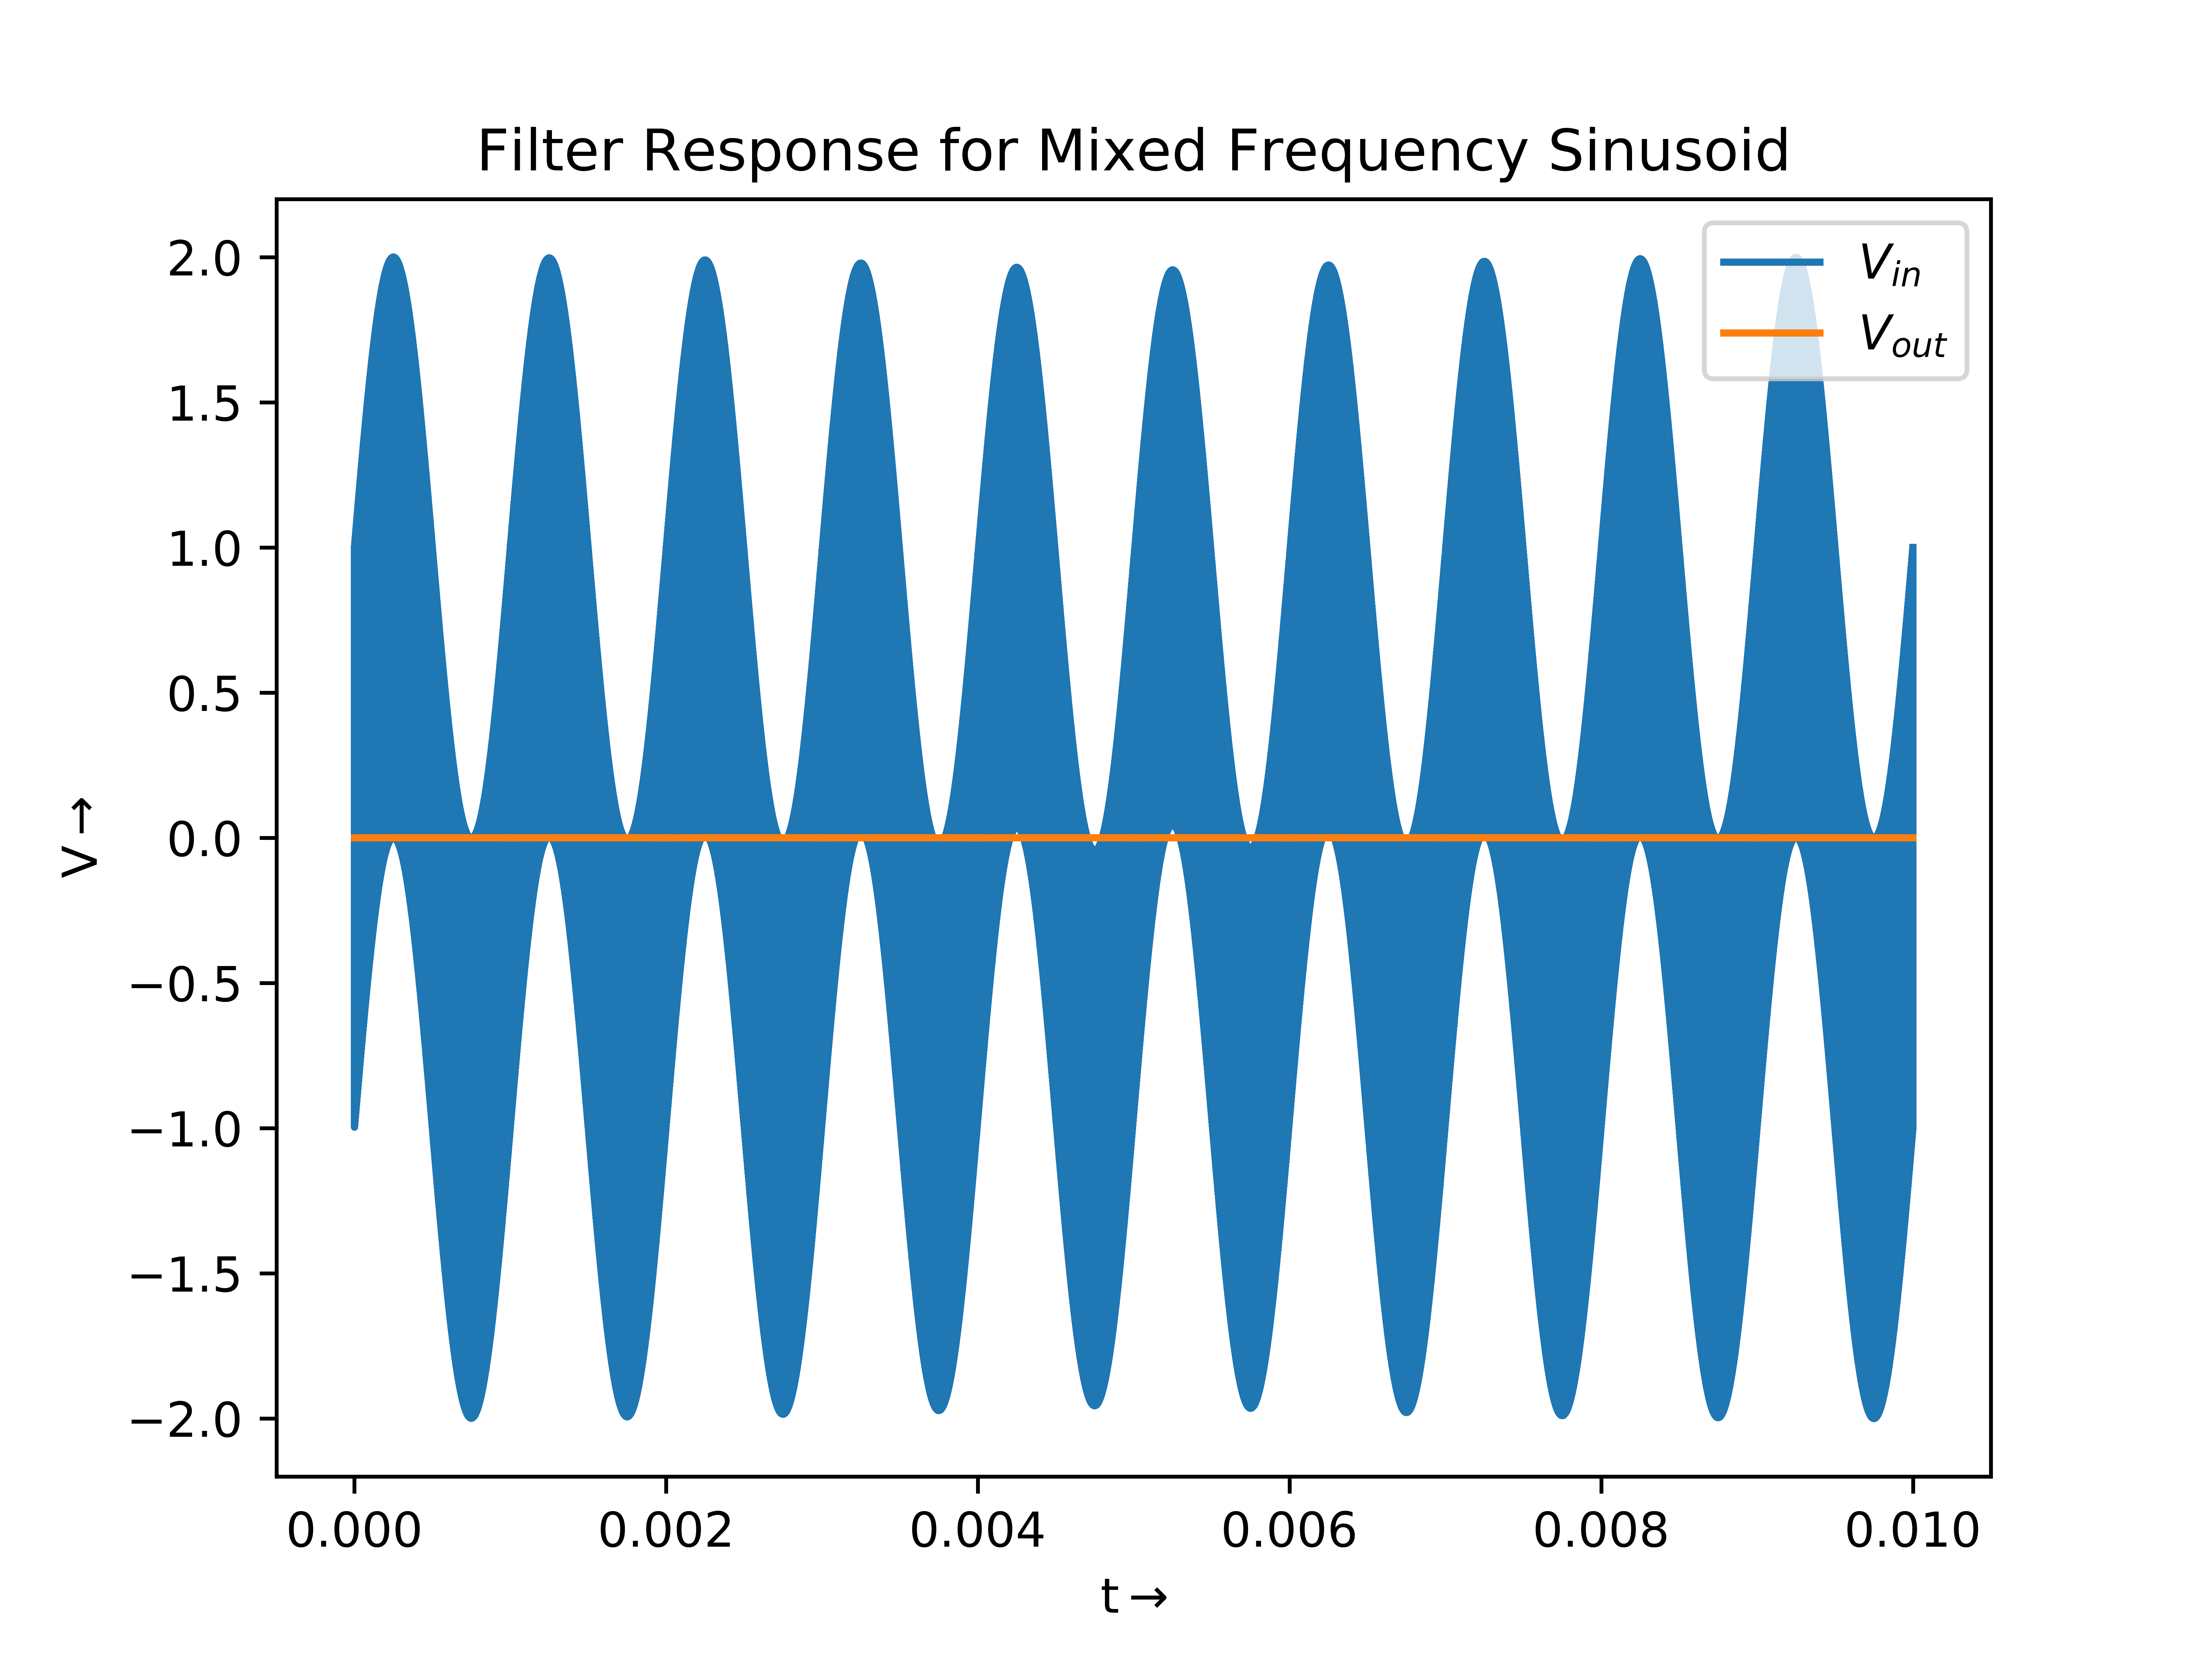
\includegraphics[scale=0.8]{images/fig2.png}
\end{center}

\pagebreak
\subsection{Question 3}

Now we will set up the High Pass Butterworth Filter and plot its magnitude response:

\begin{lstlisting}[language=Python]
G = 1.586
R1 = R3 = 1e4
C1 = C2 = 1e-9
Vi = 1
A=Matrix([[0,0,1,-1/G],[-1/(1+1/(s*R3*C2)),1,0,0],[0,-G,G,1],[s*-C1-s*C2-1/R1,s*C2,0,1/R1]])
b=Matrix([0,0,0,-Vi*s*C1])
V = A.inv()*b

# Question 3: Magnitude Response of the Filter
Vo = V[3]
H = sympy_to_lti(Vo)
omega = np.logspace(0,8,801)
ss = 1j*omega
hf = lambdify(s, Vo, 'numpy')
v = hf(ss)
plt.figure(3)
plt.loglog(omega,abs(v))
plt.xlabel(r"$\omega \rightarrow$")
plt.ylabel(r"$|H(j \omega)|\rightarrow$")
plt.grid(True)
plt.title("Magnitude Response of Butterworth Highpass Filter")
plt.savefig("images/fig3",dpi=1000)
plt.show()
\end{lstlisting}

Graph obtained:
\begin{center}
    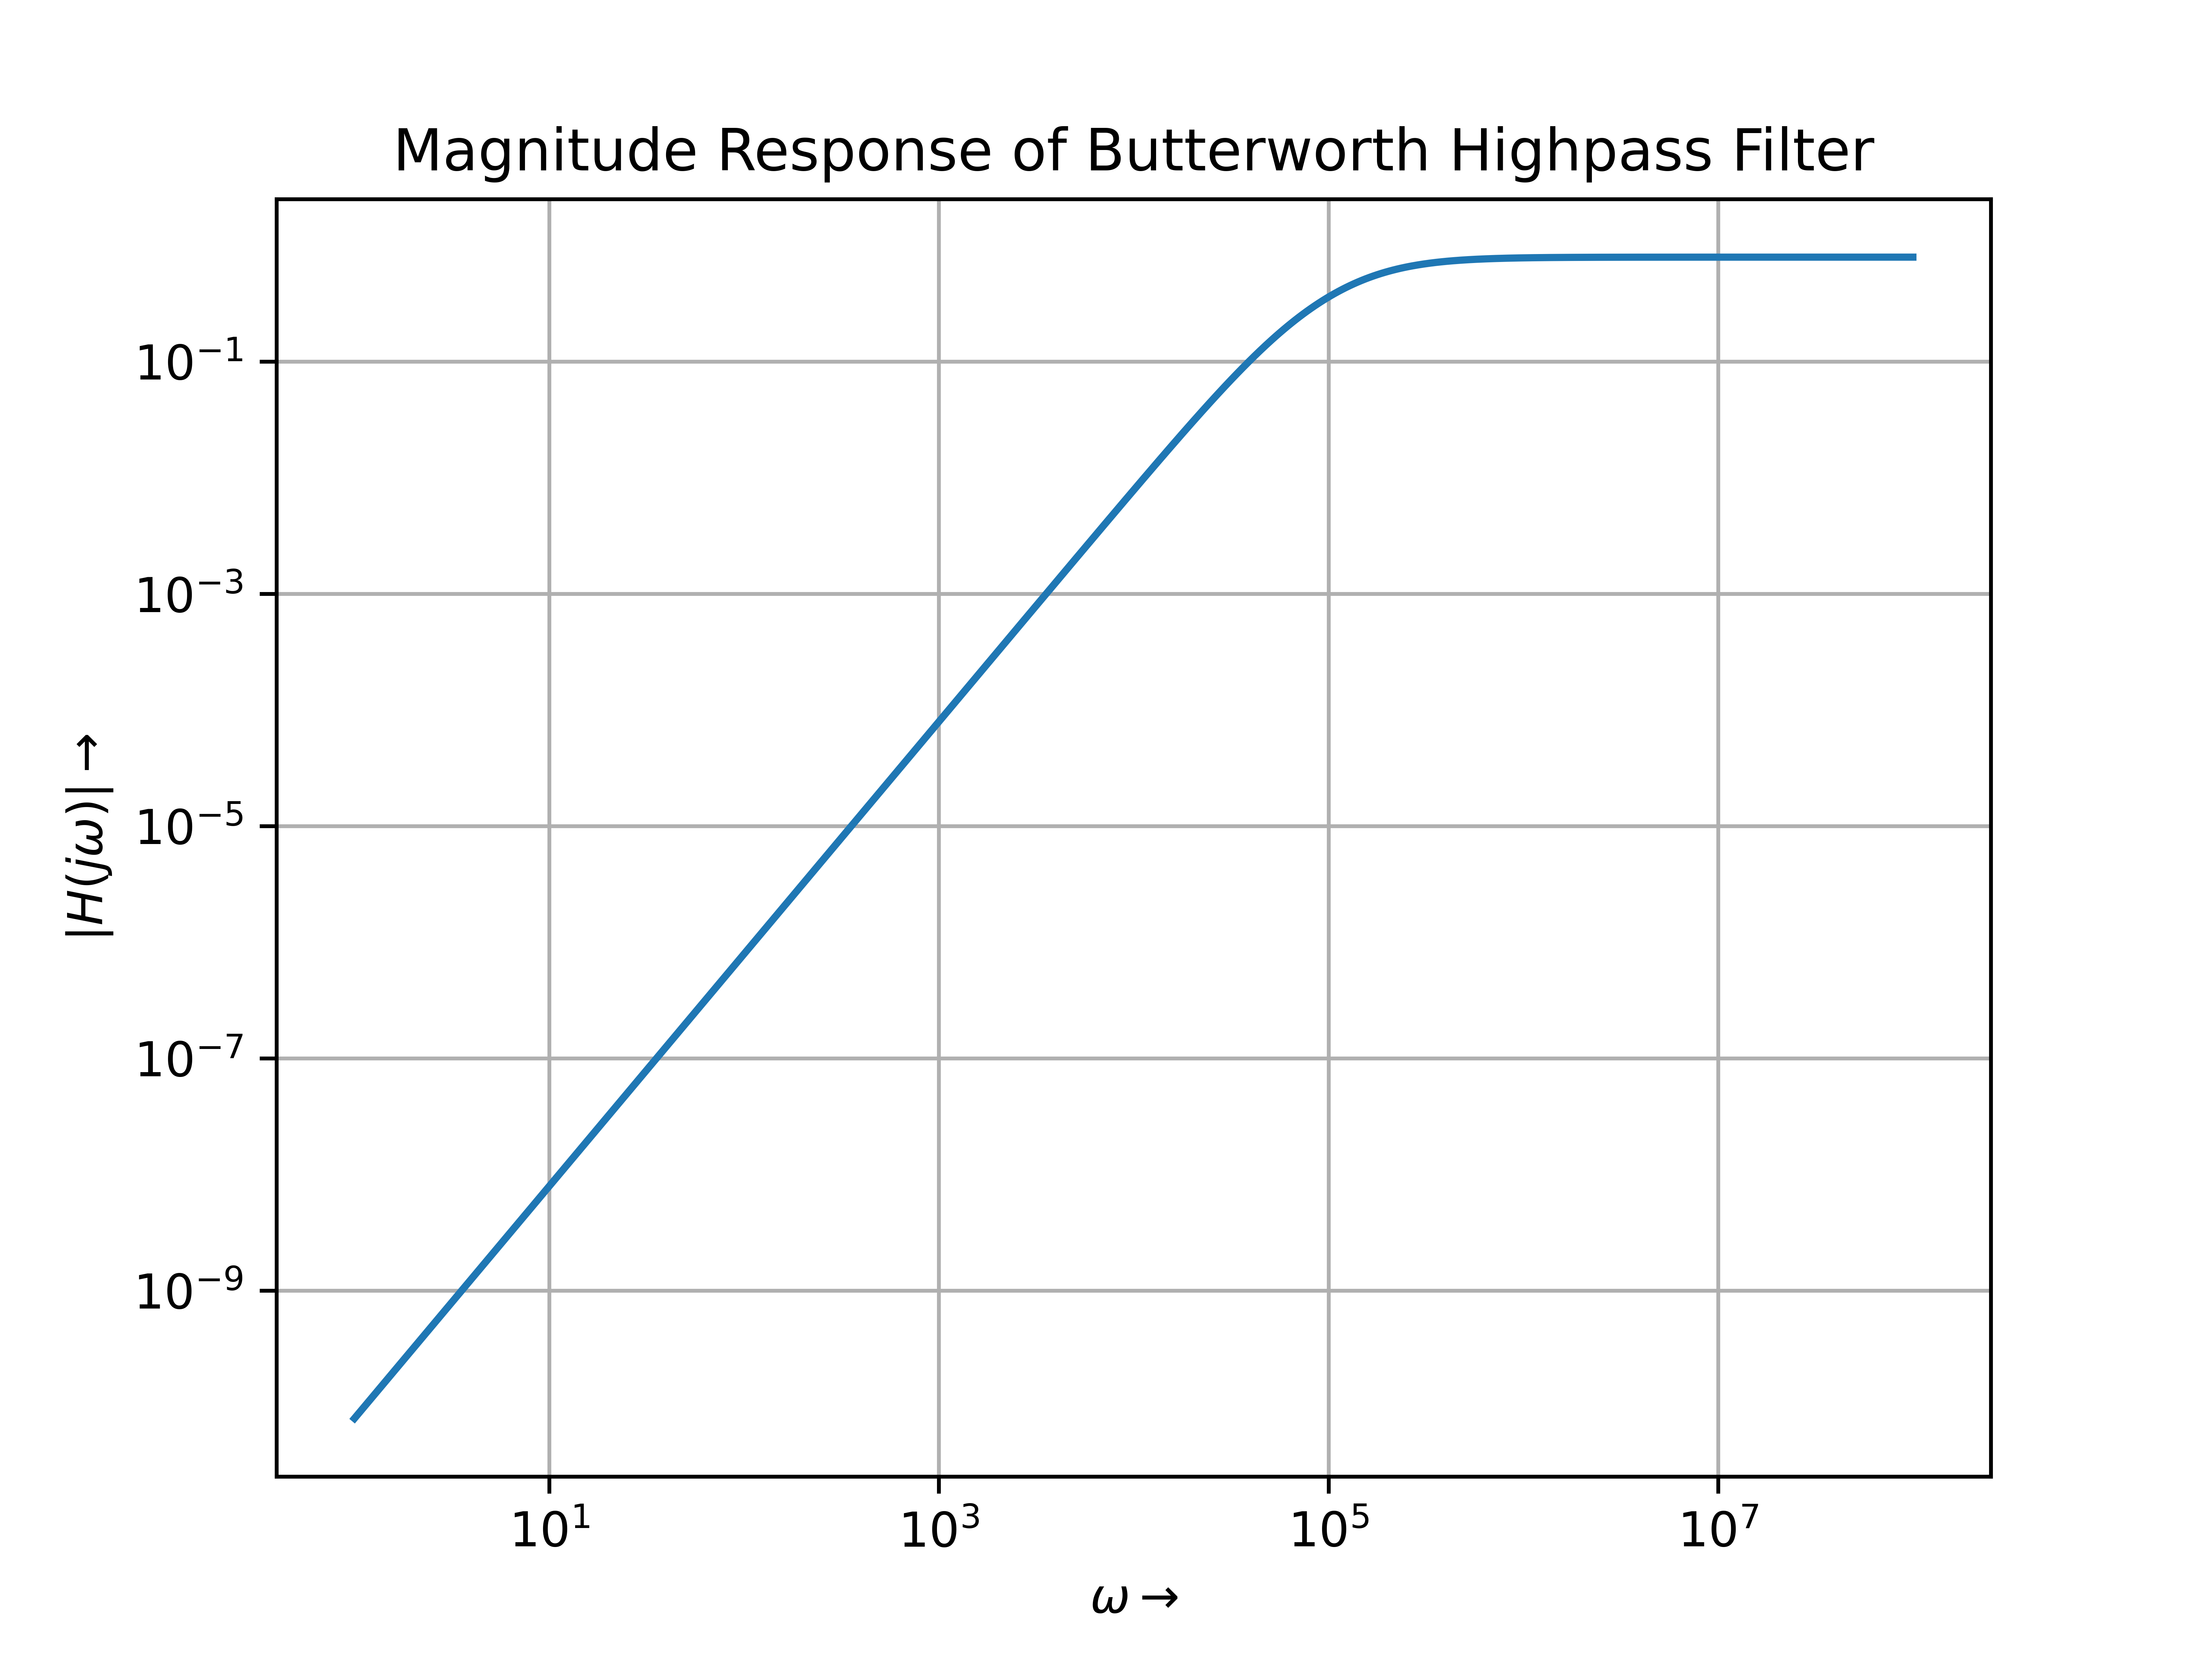
\includegraphics[scale=0.8]{images/fig3.png}
\end{center}

\pagebreak
\subsection{Question 4}

Now, we will find the response of the Highpass filter to two different damped sinusoids:

\begin{lstlisting}[language=Python]
t = np.linspace(0,10,1000)
Vi = np.multiply(np.multiply(np.exp(-0.5*t),np.sin(2*np.pi*t)),np.heaviside(t,0.5))
Vo = sp.lsim(H,Vi,T=t)
plt.figure(4)
plt.plot(Vo[0],Vi,label=r'$V_{in}$')
plt.plot(Vo[0],Vo[1],label=r'$V_{out}$')
plt.xlabel(r't$\rightarrow$')
plt.ylabel(r'$V\rightarrow$')
plt.title(r"Response for decaying sinusoid of frequency $2$ Hz")
plt.savefig("images/fig4",dpi=1000)
plt.show()

t = np.linspace(0,0.0001,10000)
Vi = np.multiply(np.multiply(np.exp(-0.5*t),np.sin(2*np.pi*200000*t)),np.heaviside(t,0.5))
Vo = sp.lsim(H,Vi,T=t)
plt.figure(5)
plt.plot(Vo[0],Vi,label=r'$V_{in}$')
plt.plot(Vo[0],Vo[1],label=r'$V_{out}$')
plt.xlabel(r't$\rightarrow$')
plt.ylabel(r'$V\rightarrow$')
plt.title(r"Response for decaying sinusoid of frequency $2 \cdot 10^5$ Hz")
plt.savefig("images/fig5",dpi=1000)
plt.show()
\end{lstlisting}
\pagebreak
Graphs obtained:
\begin{center}
    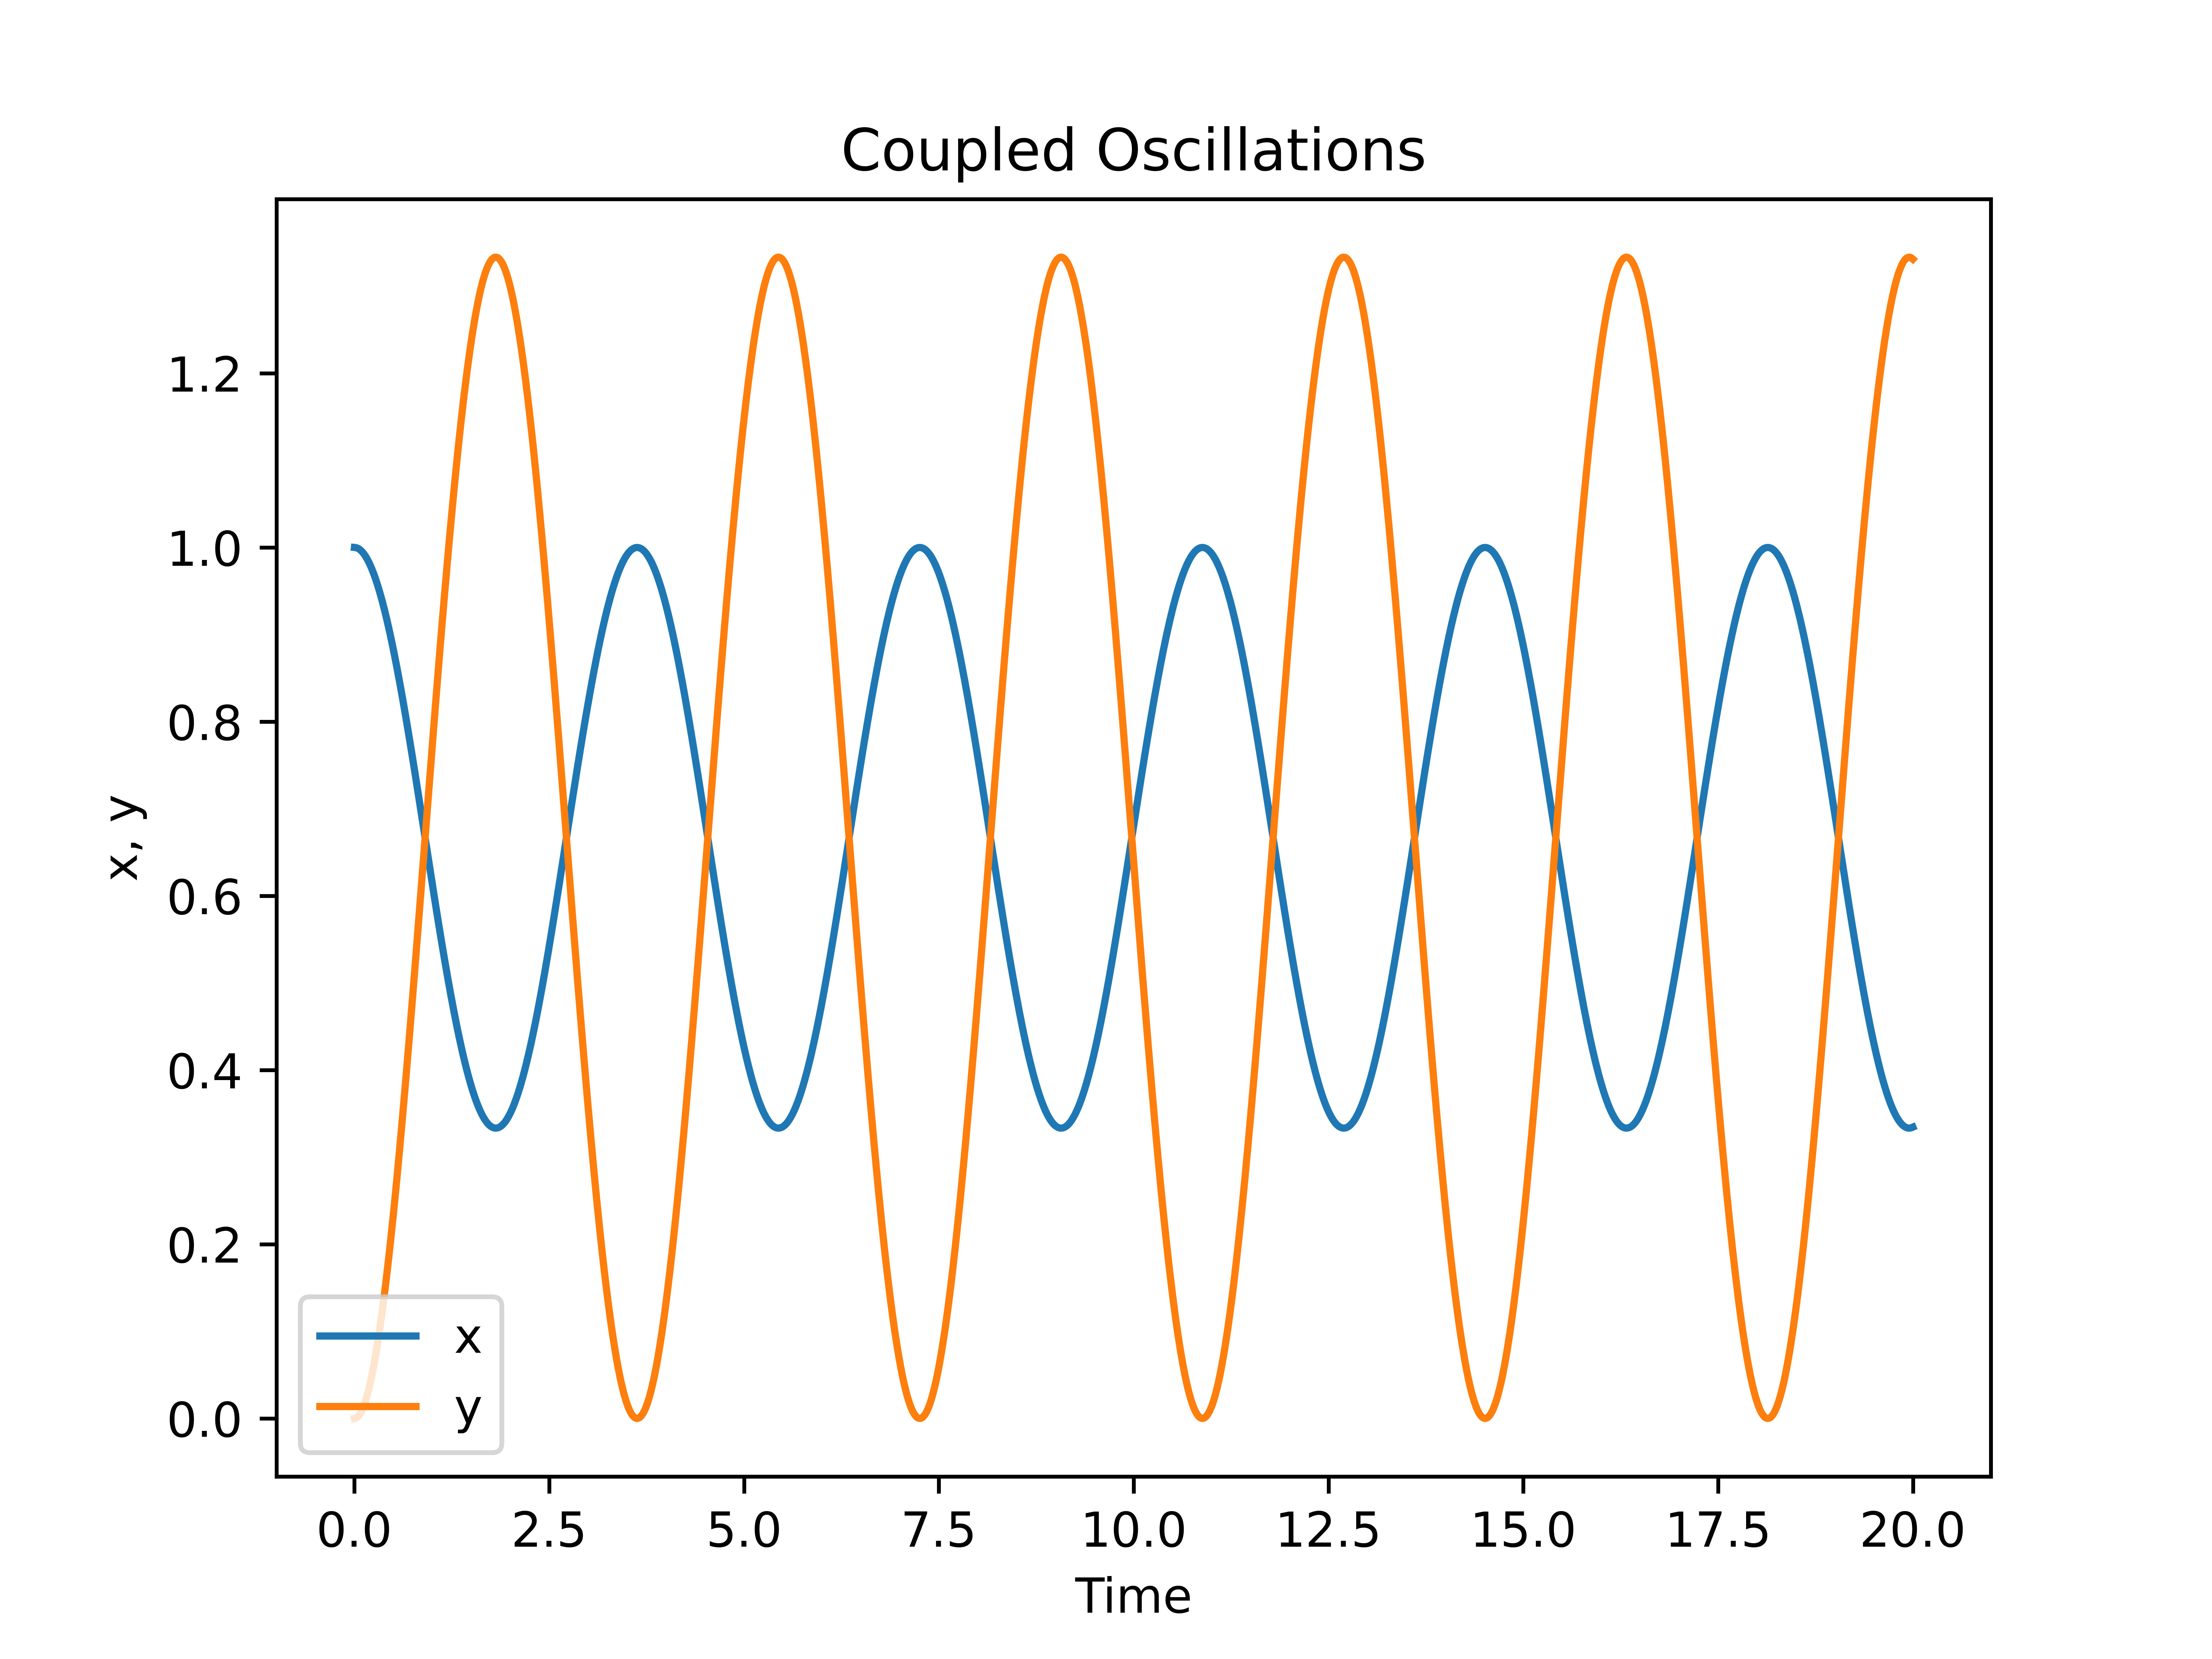
\includegraphics[scale=0.8]{images/fig4.png}
    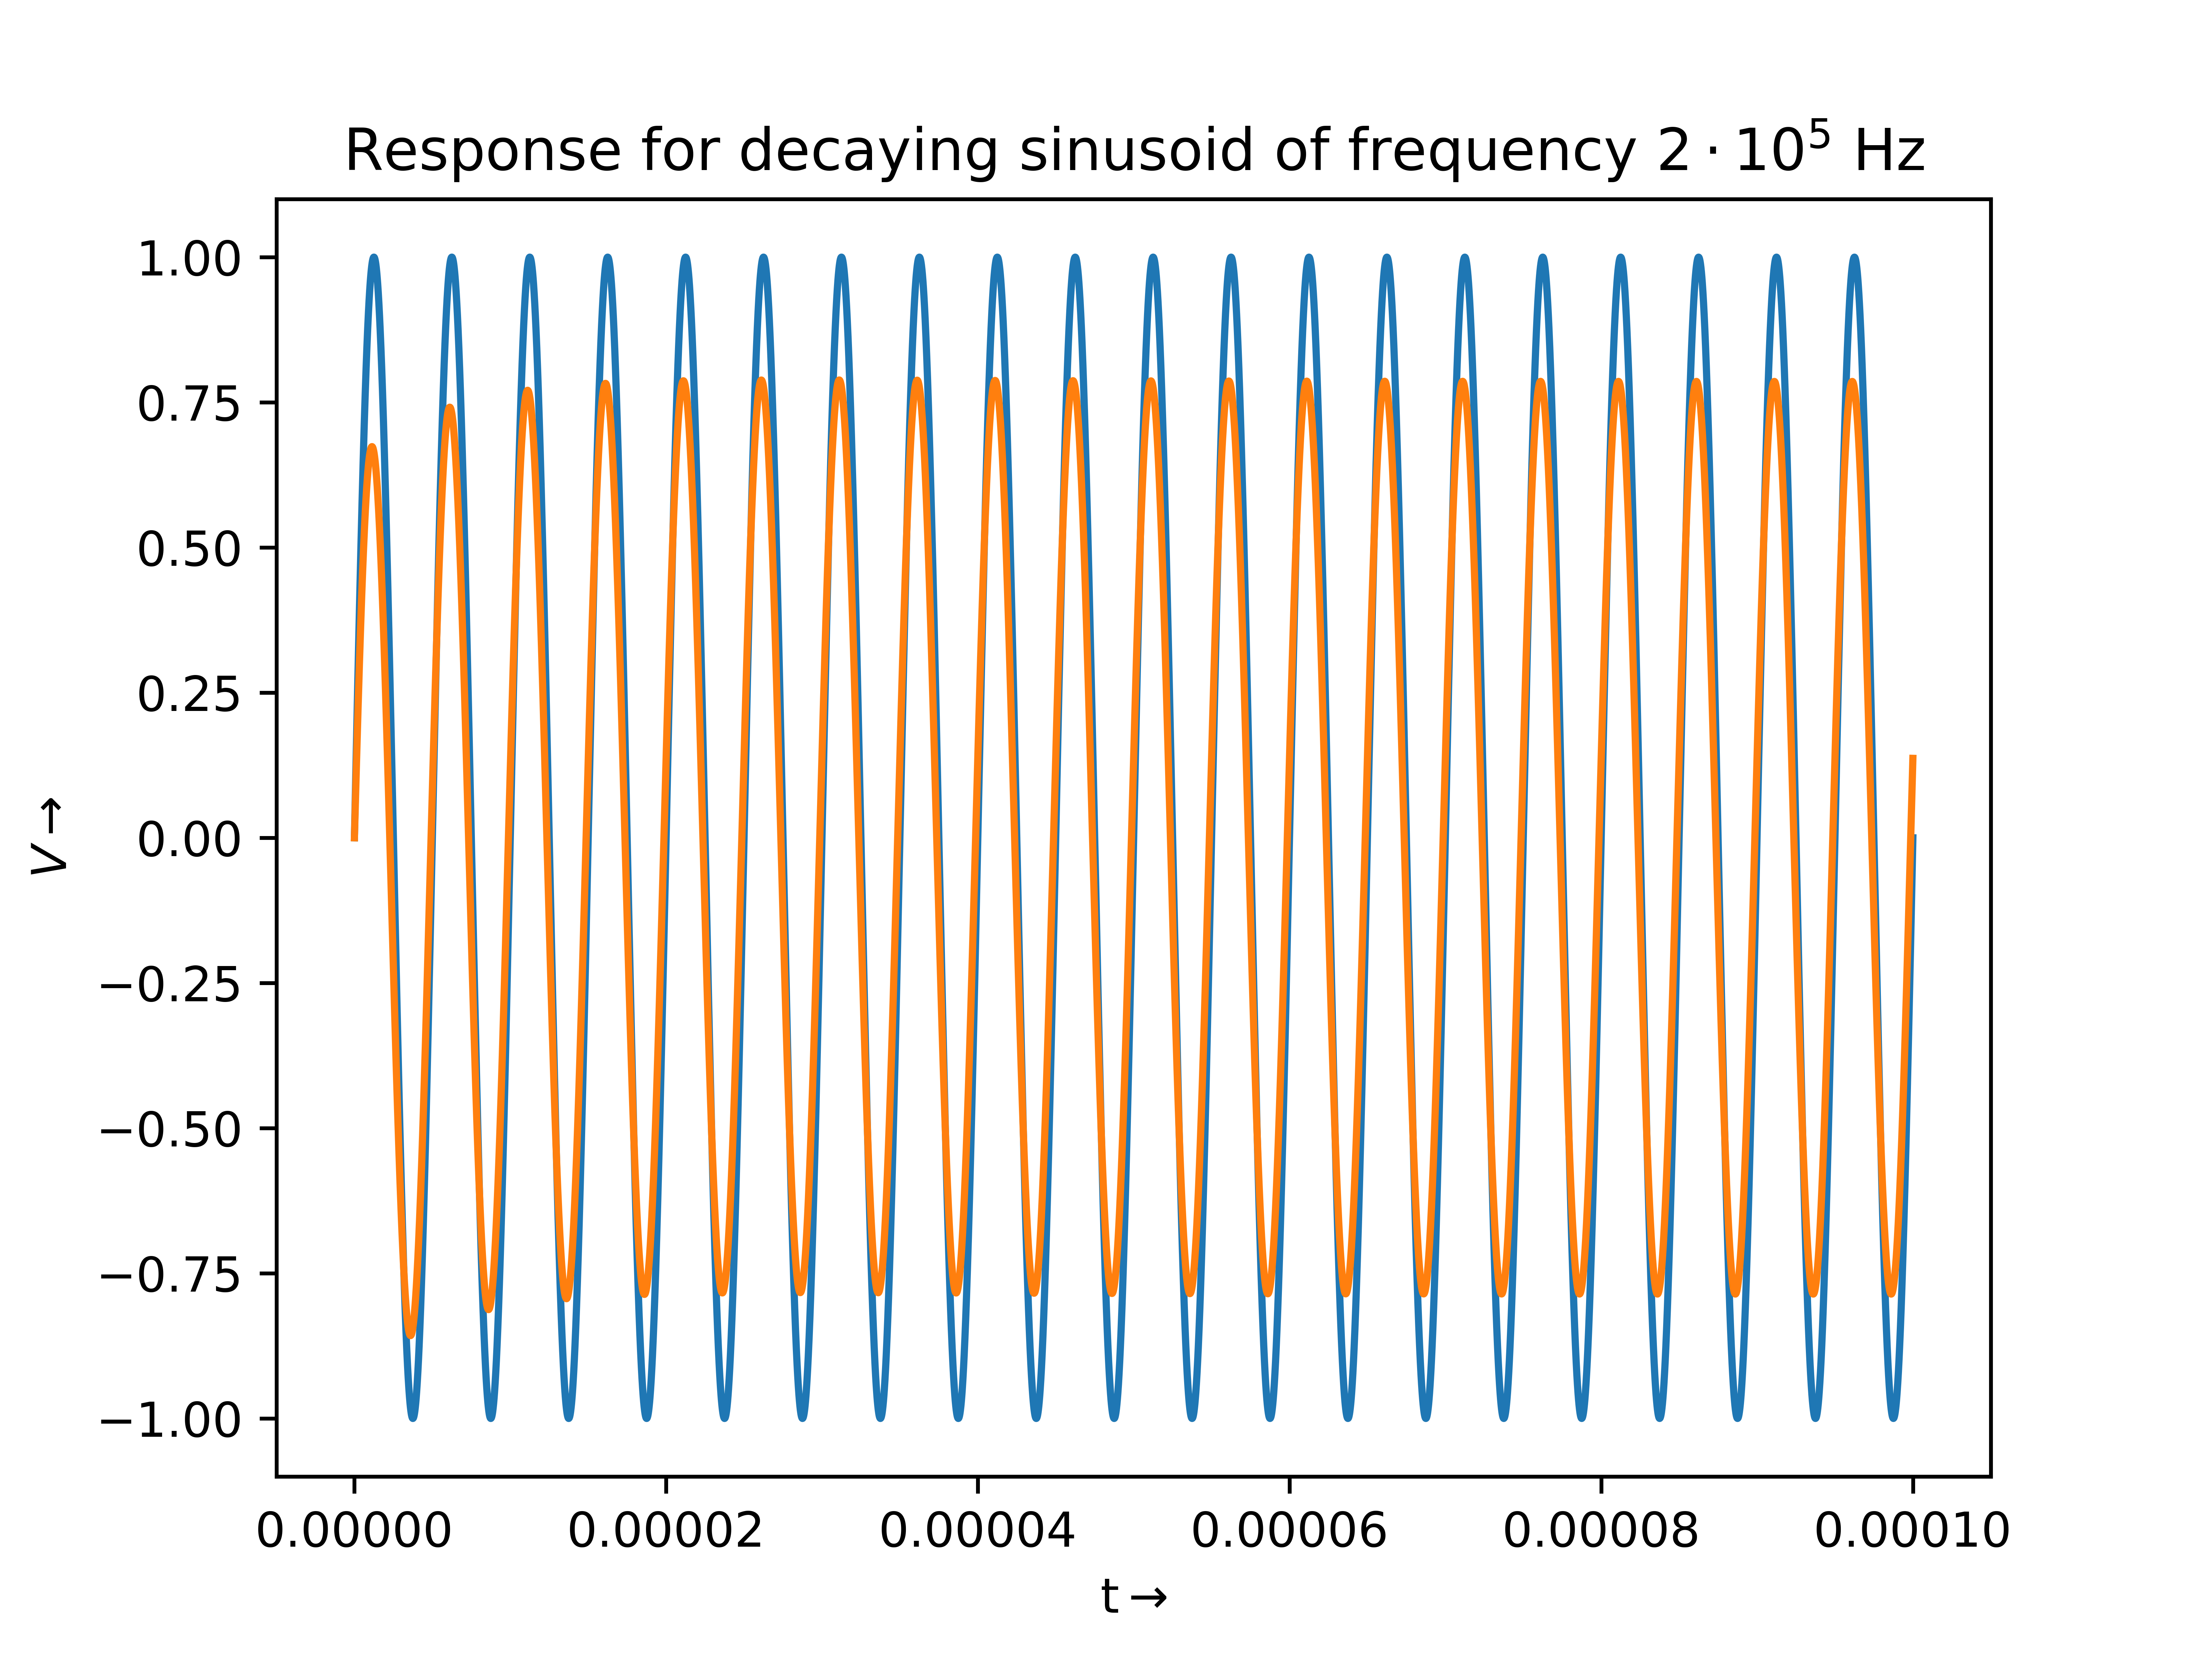
\includegraphics[scale=0.8]{images/fig5.png}
\end{center}

\pagebreak
\subsection{Question 5}

Finally, we will plot the step response of the highpass filter:

\begin{lstlisting}[language=Python]
plt.figure(6)
t = np.linspace(0,0.001,1000)
Vo = sp.step(H,T=t)
plt.plot(Vo[0],Vo[1])
plt.xlabel(r't$\rightarrow$')
plt.ylabel(r'$V_{o}\rightarrow$')
plt.title("Step Response of High Pass Butterworth Filter")
plt.savefig("images/fig6",dpi=1000)
plt.show()
\end{lstlisting}
Graph obtained:
\begin{center}
    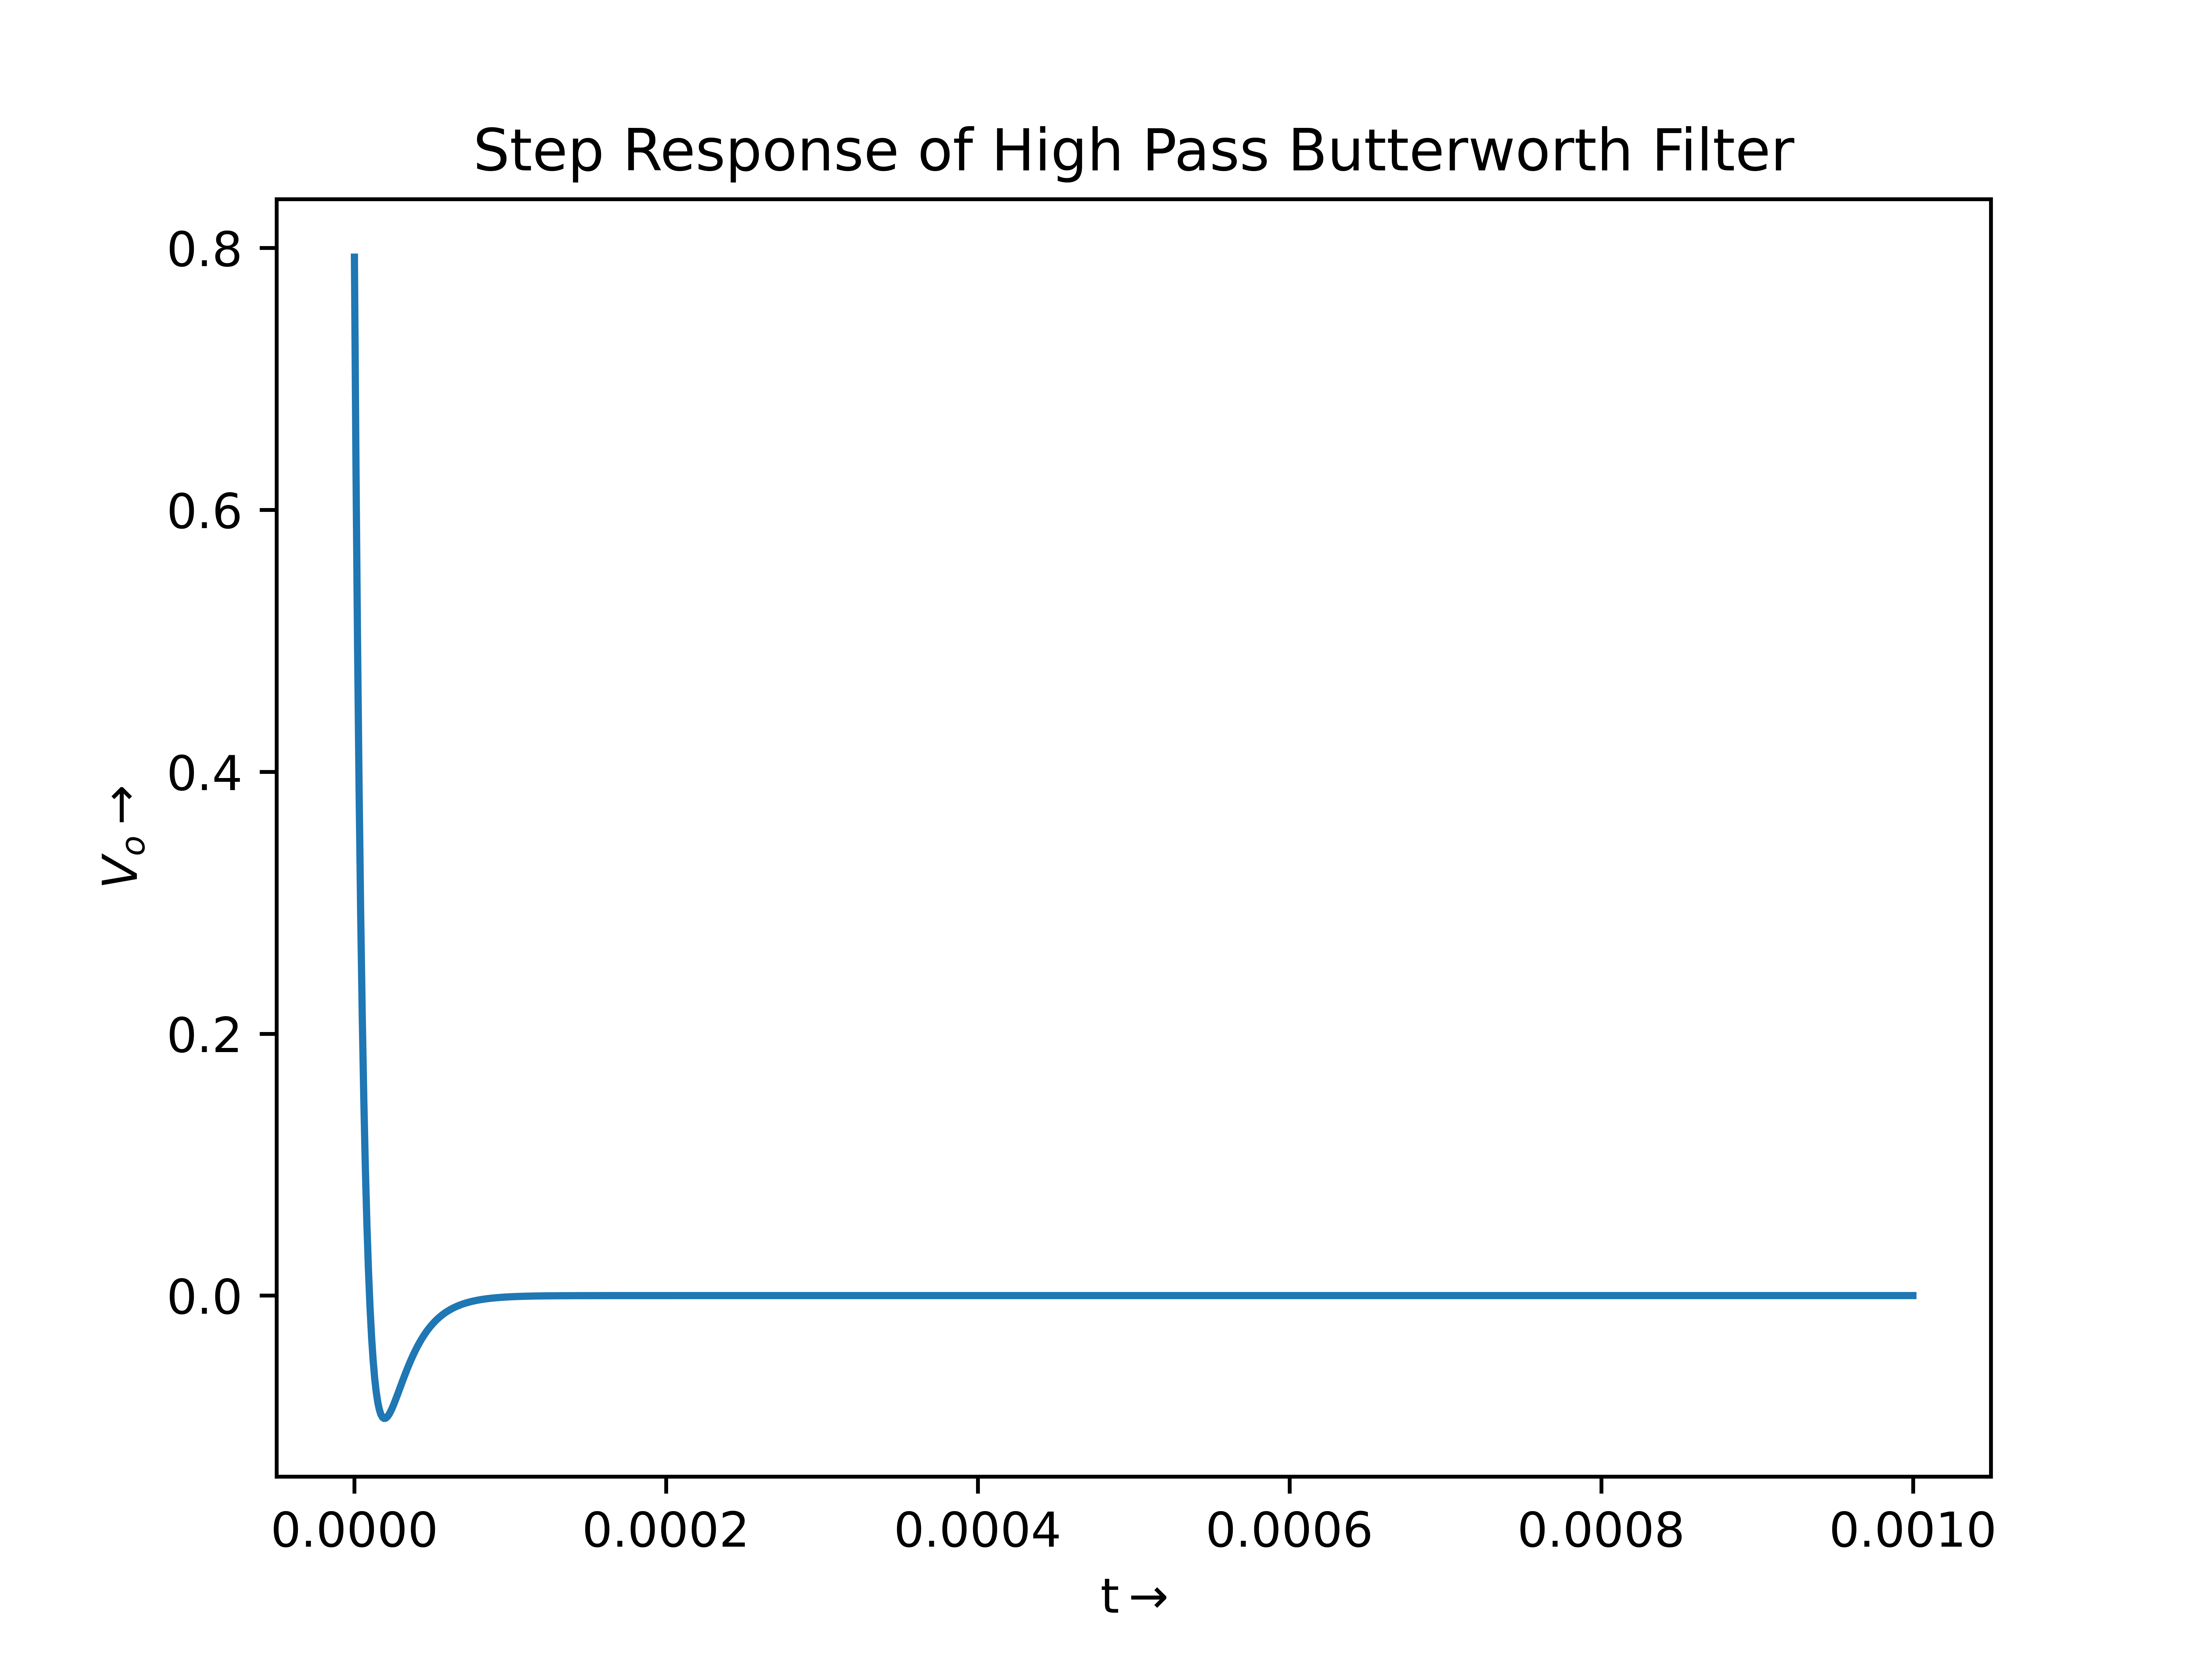
\includegraphics[scale=0.8]{images/fig6.png}
\end{center}

In this question, it was asked whether we understand the response.

The reason for the initial peak is the initial conditions. The capacitor does not allow instantaneous changes in the voltage across it. Before $t = 0$, both capacitors have no charge, and the voltage across both is 0, and this will not change instantaneously.

Referring to the circuit diagram, the instant the 1V of the unit step is applied $(t = 0^+)$, the drop across
the capacitors $C_1$ and $C_2$ will still be zero. Therefore $V_m = 1V$.

$V_m = \frac{V_o}{G}$ and $V_o = G(V_p - V_m)$, therefore we get:

$$V_o = G\left(1-\frac{V_o}{G}\right)$$
$$V_o = \frac{G}{2} = \frac{1.586}{2} = 0.793V \approx 0.8V$$

And hence, we have an initial peaking around 0.8V and then it quickly decays and settles down to the expected 0V since it is a highpass filter and DC output should hence be 0V.

\section{Conclusions}
SymPy provides an easy way to work with functions without losing generality and can be easily interfaced with SciPy and NumPy for scientific computing.

Two different filters were analyzed in this manner.
\end{document}
